%-------------------------------------------------------------------------
\section{Experiments}
\label{sec:experiments}

\subsection{Experimental Setup}

\paragraph{Architecture.}
Due to computational constraints, we conduct all experiments using a ViT-Tiny backbone with hidden
dimension $d = 192$, depth $L = 12$, $H = 3$ attention heads, MLP dimension $768$, and patch size
$P = 16$. This yields approximately 5.7M parameters across all variants and ensures that any
performance differences are attributable solely to the positional encoding mechanism. While larger
models may exhibit different absolute performance, we expect the relative trends between positional
encoding methods to generalize, as confirmed by the consistency of our findings across three
diverse tasks.

\paragraph{Training: Classification.}
Models are trained from scratch on ImageNet-100 (a 100-class subset of ImageNet-1K~\cite{deng2009imagenet}) at resolution
$224 \times 224$ for 300 epochs. We use AdamW~\cite{loshchilov2019decoupled} with base learning rate $10^{-3}$, minimum learning
rate $10^{-5}$, weight decay $0.05$, and $(\beta_1, \beta_2) = (0.9, 0.999)$. The learning rate
follows a cosine schedule with 10 epochs of linear warmup from $10^{-6}$. We apply label smoothing
with factor $0.1$, gradient clipping at norm $1.0$, and automatic mixed precision. Data
augmentation includes random resized cropping and horizontal flipping. For models with learnable
frequency parameters (RoPE and YaRN), frequency tensors and bias/normalization parameters are
excluded from weight decay.

\paragraph{Training: Detection.}
For object detection, we fine-tune on COCO 2017~\cite{lin2014microsoft} using Faster R-CNN~\cite{ren2015faster} with an FPN~\cite{lin2017feature} neck built on top of
each ViT-Tiny backbone. Models are initialized from the corresponding ImageNet-100 classification
checkpoint. Training follows standard MMDetection~\cite{chen2019mmdetection} protocols at a base resolution of $512 \times 512$.

\paragraph{Training: Segmentation.}
For semantic segmentation, we fine-tune on ADE20K~\cite{zhou2017scene} using UPerNet~\cite{xiao2018unified} with each ViT-Tiny backbone. Models
are initialized from classification checkpoints and trained following standard MMSegmentation~\cite{mmseg2020}
protocols at a base resolution of $512 \times 512$.

\paragraph{Positional Embedding Variants.}
We compare the following methods:
\begin{itemize}
    \item \textbf{Simple ViT}: Learned absolute 2D positional embeddings with bicubic interpolation at test time.
    \item \textbf{RoPE ViT}: 2D Rotary Position Embeddings with per-head random axis rotations ($\theta = 10$).
    \item \textbf{YaRN ViT}: Trained identically to RoPE (loaded from the same checkpoint); at inference, NTK-by-parts frequency scaling is applied dynamically based on the resolution ratio ($\theta = 10{,}000$, $\beta_{\text{fast}} = 32$, $\beta_{\text{slow}} = 1$).
    \item \textbf{ALiBi ViT}: Attention with Linear Biases using 2D Euclidean distance and fixed geometric head slopes. No learnable positional parameters.
    \item \textbf{FIRE ViT}: Continuous learnable attention bias parameterized by a small MLP with logarithmic distance warping and progressive interpolation.
\end{itemize}

\paragraph{Evaluation Protocol.}
For classification, we evaluate each model on the ImageNet-100 validation set at nine resolutions:
$96$, $160$, $224$ (train), $256$, $384$, $448$, $512$, $768$, and $1024$ pixels. This corresponds
to scale factors ranging from $0.43\times$ (interpolation) to $4.57\times$ (extreme extrapolation)
relative to the $14 \times 14$ training patch grid. All evaluations are performed \emph{zero-shot}
without any fine-tuning at the target resolution. For detection and segmentation, we test at
resolutions $384$, $512$ (train), $640$, $768$, and $1024$ pixels.

%-------------------------------------------------------------------------
\subsection{Classification Results}

Table~\ref{tab:classification} reports Top-1 and Top-5 accuracy across resolutions. All models peak at or
slightly above the training resolution, but diverge significantly under extrapolation.

\begin{table}[t]
\centering
\caption{Zero-shot classification accuracy (\%) on ImageNet-100 at varying resolutions. All models are trained at $224 \times 224$. Bold indicates best per resolution; underline indicates second best. YaRN uses the same checkpoint as RoPE but applies NTK-by-parts frequency scaling at inference.}
\label{tab:classification}
\resizebox{\textwidth}{!}{%
\begin{tabular}{ll|ccc|cccccc}
\toprule
& & \multicolumn{3}{c|}{\textbf{Interpolation}} & \multicolumn{6}{c}{\textbf{Extrapolation}} \\
\textbf{Model} & \textbf{Metric} & \textbf{96} & \textbf{160} & \textbf{224} & \textbf{256} & \textbf{384} & \textbf{448} & \textbf{512} & \textbf{768} & \textbf{1024} \\
& & $(0.43\times)$ & $(0.71\times)$ & $(1.0\times)$ & $(1.14\times)$ & $(1.71\times)$ & $(2.0\times)$ & $(2.29\times)$ & $(3.43\times)$ & $(4.57\times)$ \\
\midrule
\multirow{2}{*}{Simple ViT} & Top-1 & 36.62 & 63.82 & 71.94 & 72.58 & 72.50 & 72.22 & 70.08 & 60.90 & 51.42 \\
                            & Top-5 & 60.54 & 84.54 & 89.94 & 90.60 & 90.34 & 90.18 & 89.72 & 84.98 & 78.40 \\
\midrule
\multirow{2}{*}{RoPE ViT}   & Top-1 & \textbf{45.46} & \underline{70.00} & \textbf{77.30} & \textbf{78.08} & 76.46 & 72.10 & 65.90 & 36.42 & 18.90 \\
                            & Top-5 & \textbf{69.58} & \underline{87.52} & \underline{91.80} & \underline{92.60} & 92.30 & 89.92 & 86.66 & 64.04 & 42.94 \\
\midrule
\multirow{2}{*}{YaRN ViT}   & Top-1 & \underline{43.04} & \textbf{70.64} & \underline{77.28} & \underline{77.94} & \underline{77.52} & \underline{76.06} & \underline{74.52} & 64.14 & 53.44 \\
                            & Top-5 & \underline{68.00} & \textbf{88.08} & \textbf{91.80} & \textbf{92.64} & \textbf{93.34} & \underline{92.64} & \underline{91.64} & \underline{86.66} & \underline{79.12} \\
\midrule
\multirow{2}{*}{ALiBi ViT}  & Top-1 & 1.88  & 62.20 & 72.60 & 74.42 & 75.04 & 74.30 & 73.40 & \underline{68.14} & \underline{60.18} \\
                            & Top-5 & 7.86  & 83.62 & 89.48 & 90.48 & 91.30 & 91.30 & 90.60 & 88.10 & 84.16 \\
\midrule
\multirow{2}{*}{FIRE ViT}   & Top-1 & 42.28 & 65.90 & 74.48 & 76.00 & \textbf{77.88} & \textbf{77.40} & \textbf{77.22} & \textbf{71.06} & \textbf{63.14} \\
                            & Top-5 & 66.10 & 85.74 & 90.72 & 91.84 & \underline{92.94} & \textbf{93.04} & \textbf{92.94} & \textbf{91.08} & \textbf{86.80} \\
\bottomrule
\end{tabular}%
}
\end{table}

\begin{figure}[t]
    \centering
    \begin{subfigure}[b]{0.48\textwidth}
        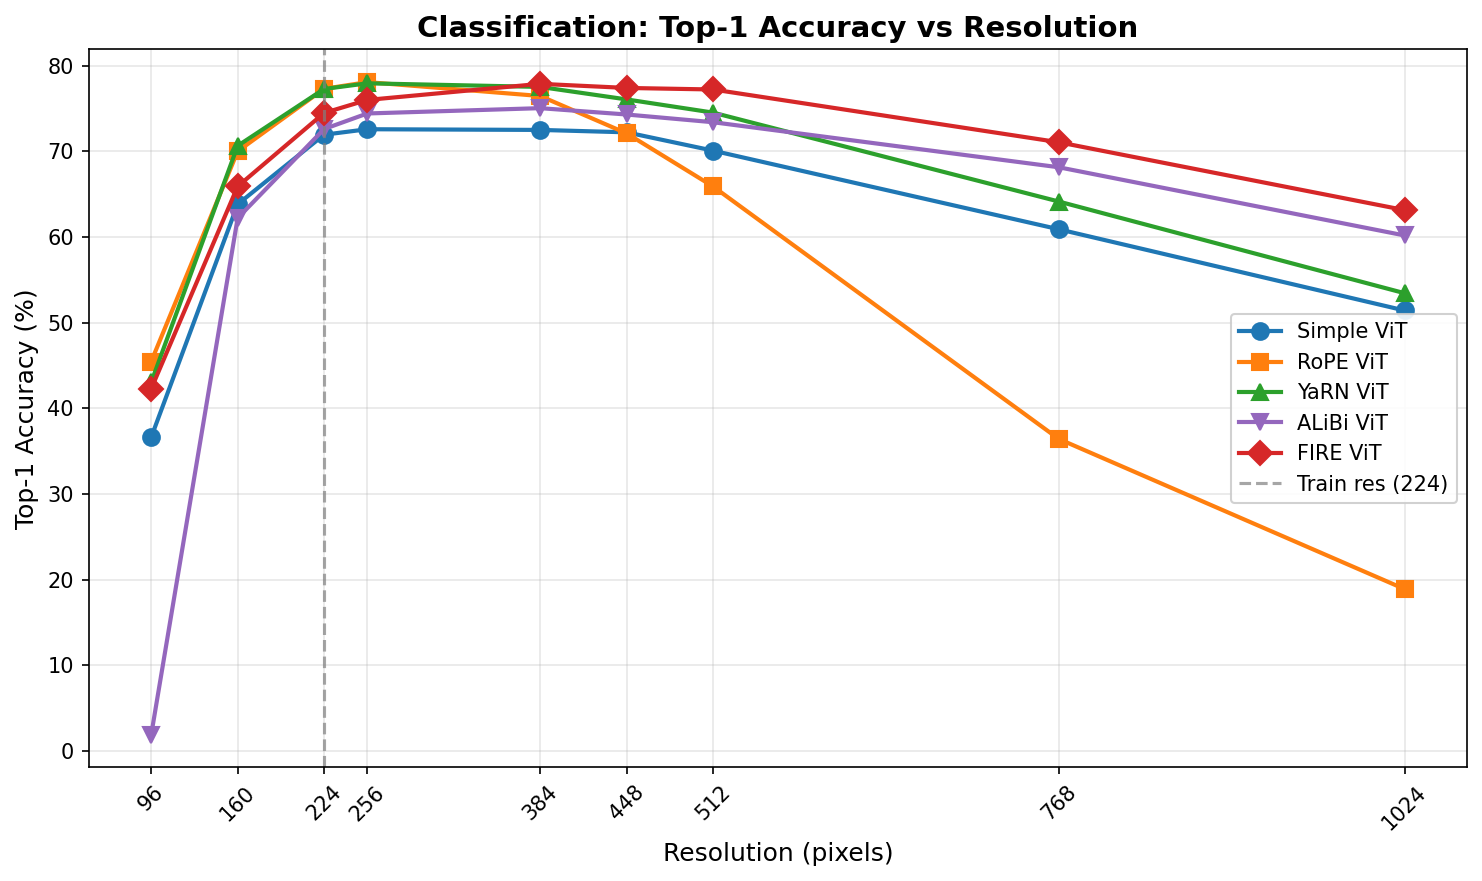
\includegraphics[width=\textwidth]{results/extrapolation_top1_vs_resolution.png}
        \caption{Top-1 Accuracy vs.\ Resolution}
        \label{fig:top1}
    \end{subfigure}
    \hfill
    \begin{subfigure}[b]{0.48\textwidth}
        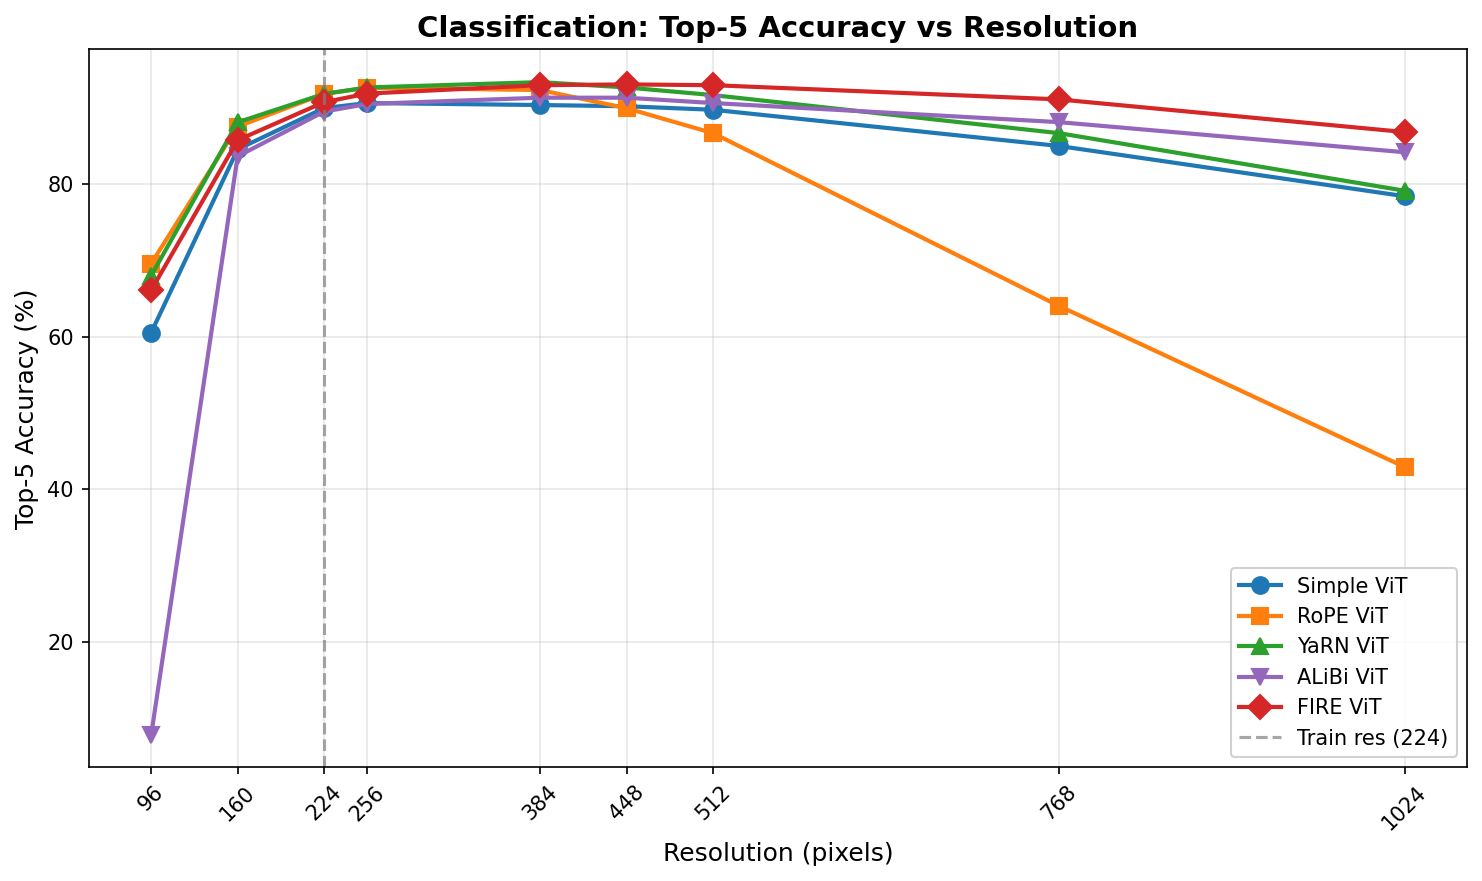
\includegraphics[width=\textwidth]{results/extrapolation_top5_vs_resolution.png}
        \caption{Top-5 Accuracy vs.\ Resolution}
        \label{fig:top5}
    \end{subfigure}
    \caption{Zero-shot classification extrapolation on ImageNet-100. All models are trained at $224\times224$ (dashed line) and evaluated up to $1024\times1024$ without fine-tuning. FIRE ViT and ALiBi ViT exhibit the most robust extrapolation behavior, while raw RoPE ViT degrades sharply beyond the training resolution.}
    \label{fig:classification_extrapolation}
\end{figure}

Figure~\ref{fig:classification_extrapolation} visualizes these trends. While RoPE ViT attains the
highest accuracy near the training resolution, FIRE ViT and ALiBi ViT remain substantially more
stable under extreme resolution scaling.

\paragraph{Key Observations.}
\textbf{(i) Bias-based methods extrapolate best.} FIRE ViT achieves the highest accuracy at every
resolution above $384$, retaining $63.14\%$ at $1024$ (only $11.34$ pp below its $224$ baseline).
ALiBi ViT exhibits a similarly graceful degradation profile, dropping just $12.42$ pp from $224$ to
$1024$. Both methods model relative distance through additive attention biases that are inherently
resolution-agnostic.

\textbf{(ii) Raw RoPE collapses at high extrapolation.} RoPE ViT achieves the best accuracy at the
training resolution ($77.30\%$) but degrades catastrophically under extrapolation, falling to
$18.90\%$ at $1024$, a $58.40$ pp drop. This is consistent with the known sensitivity of RoPE to
out-of-distribution positional frequencies.

\textbf{(iii) YaRN significantly improves over raw RoPE.} YaRN's NTK-by-parts scaling yields substantial gains over raw RoPE across all extrapolation regimes. At moderate extrapolation ($77.52\%$ vs.\ $76.46\%$ at $384$), the improvement is modest, but at extreme scales the gap widens dramatically: YaRN retains $53.44\%$ at $1024$ compared to RoPE's $18.90\%$, a $34.54$ pp advantage. This demonstrates that selective frequency scaling is highly effective for rotation-based methods, though YaRN still falls short of bias-based methods (FIRE: $63.14\%$, ALiBi: $60.18\%$) at the largest scale.

\textbf{(iv) Simple ViT is surprisingly competitive.} Bicubic interpolation of learned absolute
embeddings provides a strong baseline, outperforming raw RoPE and YaRN at high extrapolation
while remaining worse than ALiBi and FIRE.

%-------------------------------------------------------------------------
\subsection{Detection Results}

Table~\ref{tab:detection_map} reports zero-shot bbox mAP on COCO under resolution extrapolation.
Detection models are trained at $512 \times 512$ and evaluated at resolutions up to $1024$.

\begin{table}[t]
\centering
\caption{Detection performance (\%) on COCO at varying resolutions. Trained at $512 \times 512$. AP$_{50}$ provides a more interpretable view of the extrapolation trends.}
\label{tab:detection_map}
\small
\begin{tabular}{ll|ccccc}
\toprule
\textbf{Model} & \textbf{Metric} & \textbf{384} & \textbf{512} & \textbf{640} & \textbf{768} & \textbf{1024} \\
\midrule
\multirow{2}{*}{Simple ViT} & mAP & 3.7 & 5.6 & 3.5 & 3.3 & 2.5 \\
                            & AP$_{50}$ & 8.4 & 12.8 & 8.0 & 7.3 & 5.5 \\
\midrule
\multirow{2}{*}{RoPE ViT}   & mAP & 6.0 & 6.8 & 6.0 & 4.5 & 1.6 \\
                            & AP$_{50}$ & 13.2 & 15.1 & 13.7 & 10.4 & 3.7 \\
\midrule
\multirow{2}{*}{YaRN ViT}   & mAP & 6.0 & 6.8 & 6.1 & 4.8 & 2.7 \\
                            & AP$_{50}$ & 13.0 & 15.1 & 13.9 & 11.2 & 6.2 \\
\midrule
\multirow{2}{*}{ALiBi ViT}  & mAP & 3.0 & 3.4 & 3.4 & 3.3 & 2.7 \\
                            & AP$_{50}$ & 6.6 & 7.6 & 7.6 & 7.2 & 5.9 \\
\midrule
\multirow{2}{*}{FIRE ViT}   & mAP & 3.4 & 3.4 & 3.2 & 2.9 & 2.3 \\
                            & AP$_{50}$ & 7.4 & 7.5 & 6.8 & 6.1 & 4.7 \\
\bottomrule
\end{tabular}
\end{table}

In detection, RoPE ViT achieves the highest mAP at the training resolution ($6.8\%$) but
experiences the steepest decline, dropping to $1.6\%$ at $1024$, a $75\%$ relative drop in AP$_{50}$ (from $15.1\%$ to $3.7\%$). ALiBi ViT demonstrates the
most stable extrapolation profile, with only a $22\%$ relative drop in AP$_{50}$ from $512$ to $1024$. Notably, the
overall mAP values are low due to the limited capacity of ViT-Tiny and training on ImageNet-100
rather than full ImageNet-1K; however, the \emph{relative} degradation patterns are consistent with
the classification findings and confirm that positional encoding robustness transfers to dense
prediction.

\paragraph{Object Size Breakdown.}
Figure~\ref{fig:object_size} decomposes detection performance by object scale (small, medium, large).
A striking finding is that \emph{large objects degrade most rapidly} under extrapolation across all methods.
At $1024$ px, mAP$_L$ collapses to near-zero for most methods ($<0.01$), while mAP$_S$ for small objects
actually \emph{increases} for bias-based methods: ALiBi reaches $5.0\%$ and FIRE reaches $4.5\%$.
This counterintuitive result suggests that higher resolution provides more pixels per small object,
improving detection, while large objects suffer from attention pattern fragmentation.
RoPE exhibits the most severe large-object collapse ($9.0\% \to 0.1\%$), whereas ALiBi maintains
the most balanced performance across scales.

\begin{figure}[t]
    \centering
    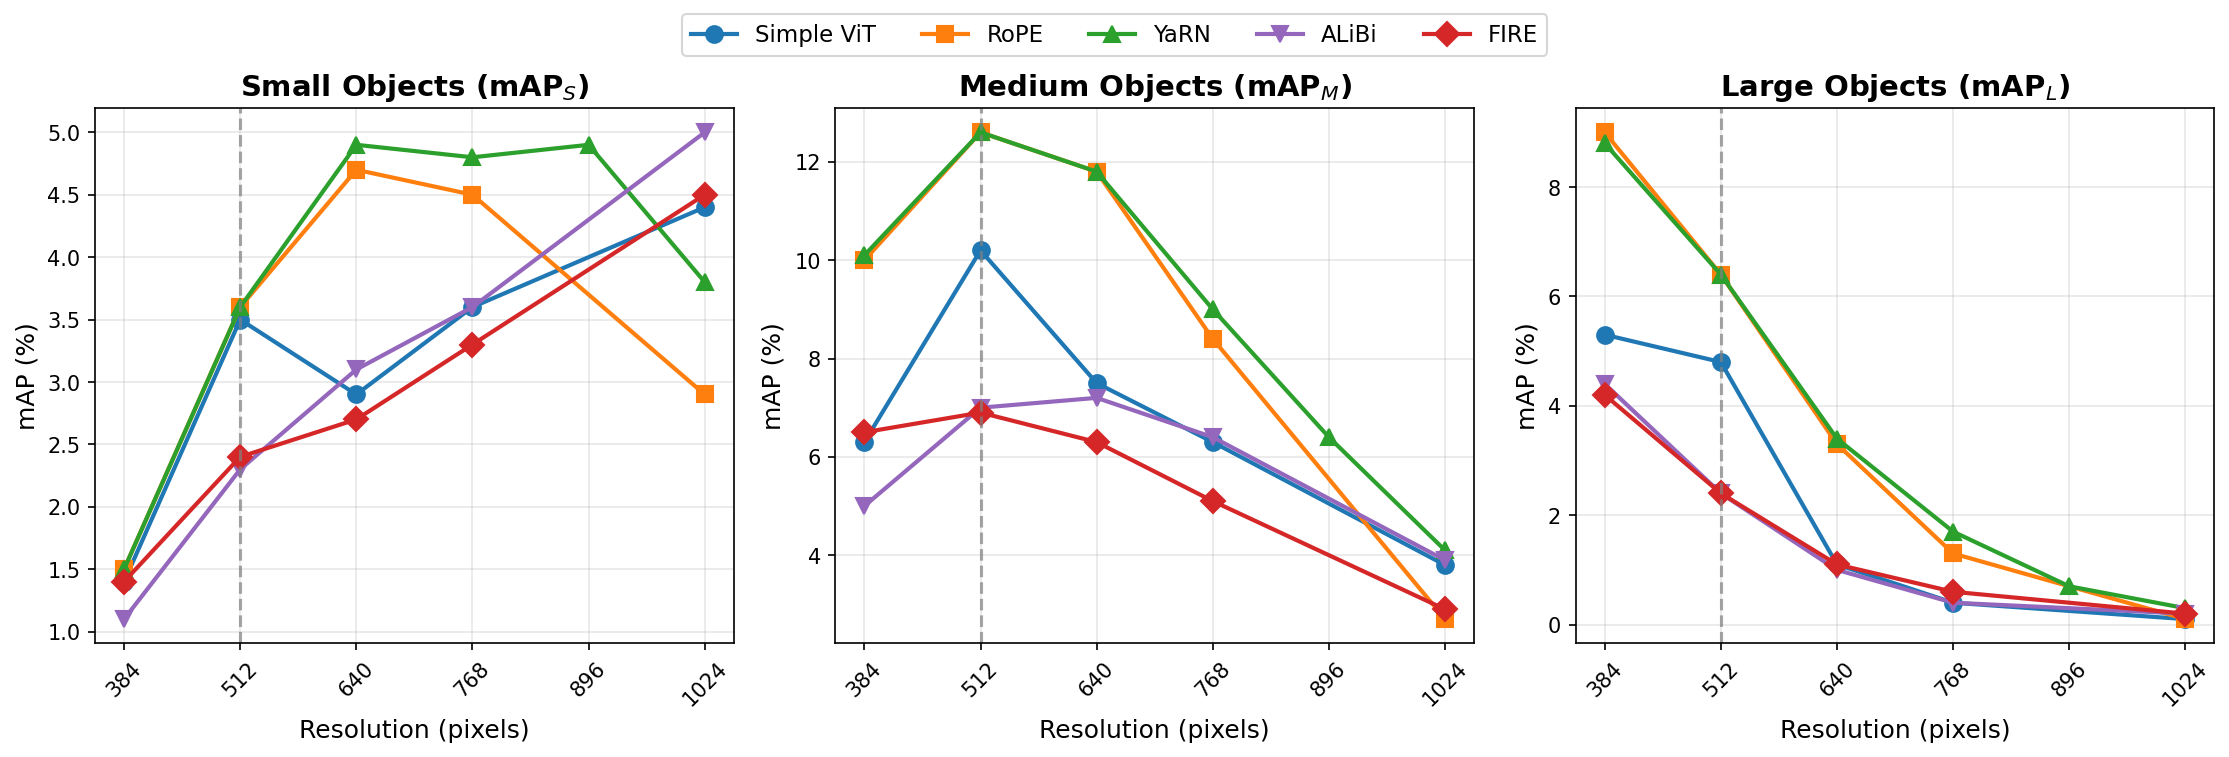
\includegraphics[width=\columnwidth]{figures/detection_object_size_breakdown.png}
    \caption{Detection mAP breakdown by object size across resolutions. Large objects (mAP$_L$) degrade most rapidly under extrapolation, while small object detection (mAP$_S$) improves at higher resolutions for bias-based methods.}
    \label{fig:object_size}
\end{figure}

%-------------------------------------------------------------------------
\subsection{Segmentation Results}

Table~\ref{tab:segmentation_miou} reports mIoU on ADE20K under resolution extrapolation.

\begin{table}[t]
\centering
\caption{Segmentation mIoU (\%) on ADE20K at varying resolutions. Trained at $512 \times 512$.}
\label{tab:segmentation_miou}
\small
\begin{tabular}{l|ccccc}
\toprule
\textbf{Model} & \textbf{384} & \textbf{512} & \textbf{640} & \textbf{768} & \textbf{1024} \\
\midrule
Simple ViT & 16.5 & 21.8 & 16.0 & 14.5 & 11.5 \\
RoPE ViT   & \underline{24.5} & \textbf{25.0} & 23.1 & 19.3 & 9.2 \\
YaRN ViT   & \textbf{24.6} & \underline{24.9} & \underline{23.7} & \underline{20.9} & 15.4 \\
ALiBi ViT  & 22.2 & 23.5 & 23.6 & \textbf{23.0} & \textbf{20.5} \\
FIRE ViT   & 23.4 & 24.4 & \textbf{24.2} & 22.5 & \underline{19.8} \\
\bottomrule
\end{tabular}
\end{table}

Segmentation results reinforce the classification trends. ALiBi ViT retains $20.5\%$ mIoU at
$1024$ (only $3.0$ pp below its peak), while RoPE ViT degrades from $25.0\%$ to $9.2\%$, a
$15.8$ pp collapse. FIRE ViT similarly maintains strong performance, dropping only $4.6$ pp from
peak to $1024$. Simple ViT suffers a $10.3$ pp decline, confirming that interpolated absolute
embeddings provide weaker spatial coherence than relative or bias-based alternatives for dense
prediction at novel resolutions.

\begin{figure}[t]
    \centering
    \begin{subfigure}[b]{0.48\textwidth}
        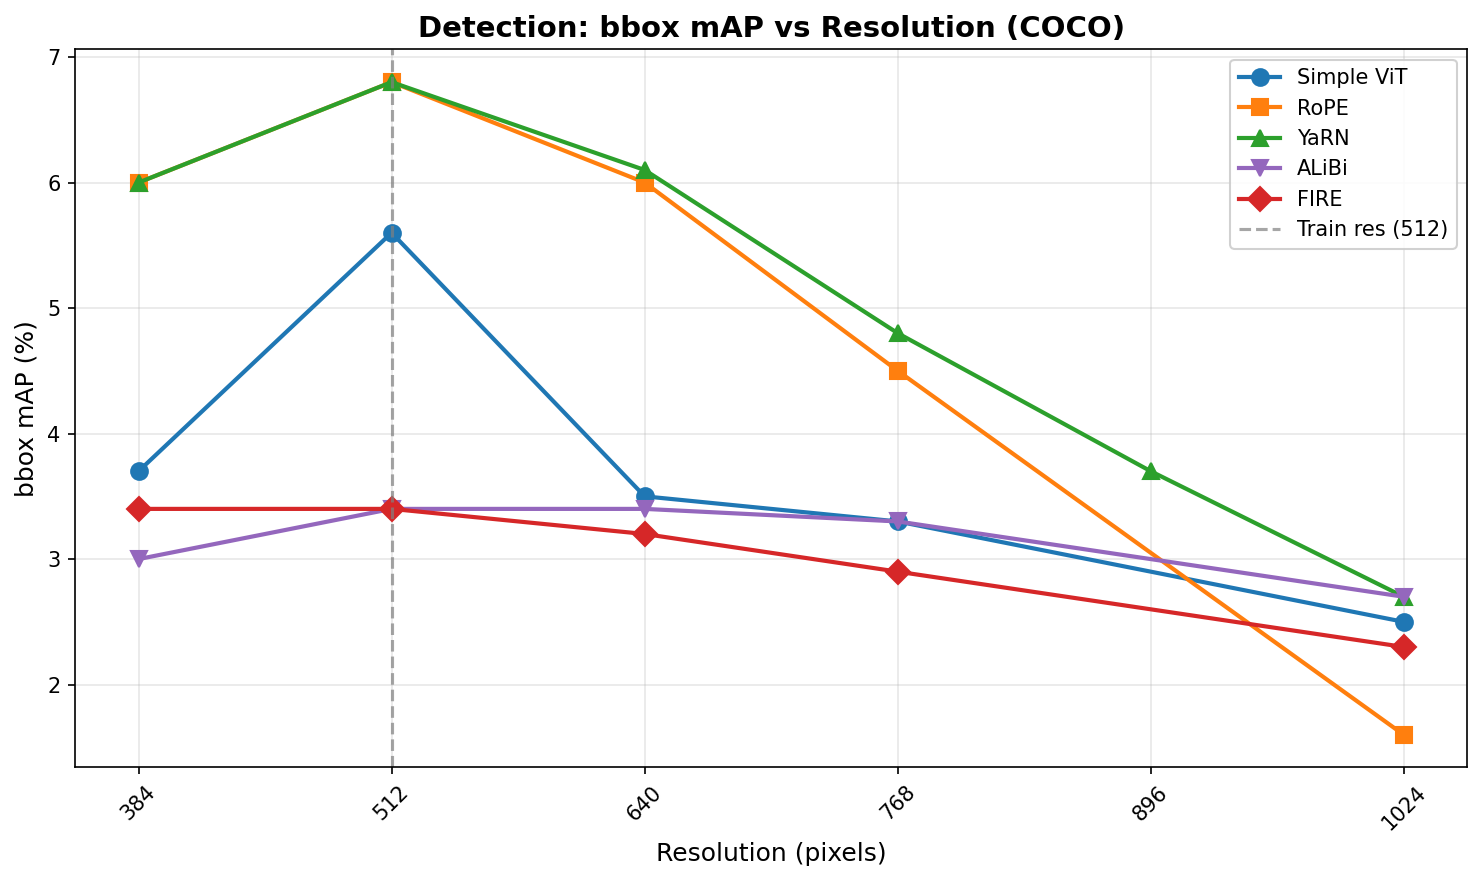
\includegraphics[width=\textwidth]{results/detection_extrapolation_map_vs_resolution.png}
        \caption{COCO bbox mAP vs.\ Resolution}
        \label{fig:detection_curve}
    \end{subfigure}
    \hfill
    \begin{subfigure}[b]{0.48\textwidth}
        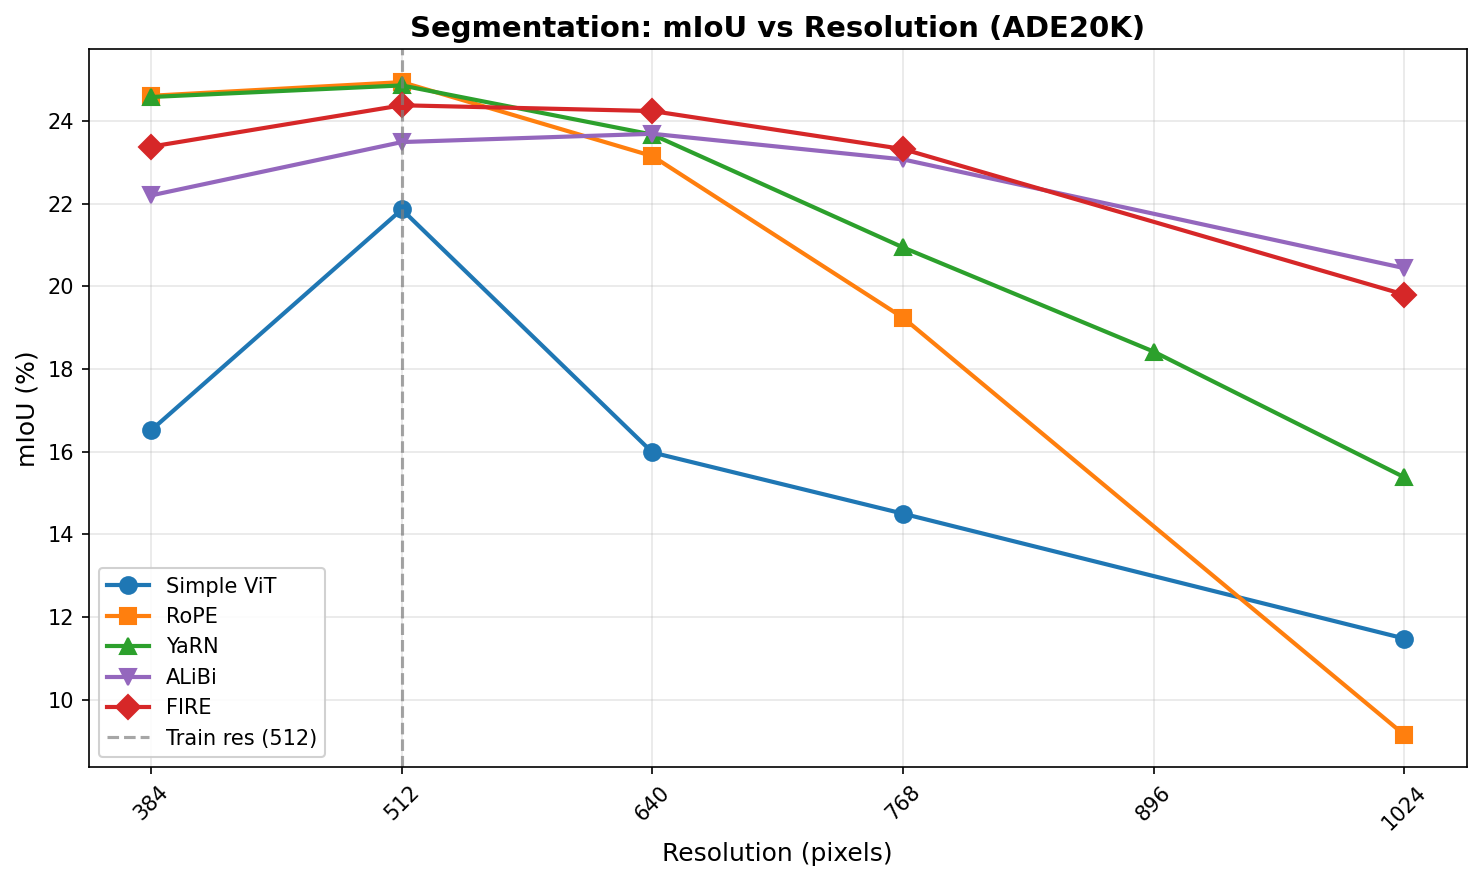
\includegraphics[width=\textwidth]{results/segmentation_extrapolation_miou_vs_resolution.png}
        \caption{ADE20K mIoU vs.\ Resolution}
        \label{fig:segmentation_curve}
    \end{subfigure}
    \caption{Zero-shot extrapolation on dense prediction tasks. All models are trained at $512\times512$ (dashed line) and evaluated up to $1024\times1024$ without fine-tuning. ALiBi ViT and FIRE ViT maintain stable performance at higher resolutions, while RoPE ViT degrades sharply. YaRN provides moderate improvement over RoPE but still degrades at extreme scales.}
    \label{fig:dense_extrapolation}
\end{figure}

Figure~\ref{fig:dense_extrapolation} shows that the extrapolation trends observed in classification
transfer to dense prediction tasks as well. Relative-bias methods remain substantially more stable
than rotation-based methods as evaluation resolution increases.

%-------------------------------------------------------------------------
\subsection{Analysis}

\paragraph{Bias vs.\ Rotation Methods.}
Across all three tasks, the additive bias methods (ALiBi and FIRE) consistently outperform the
multiplicative rotation methods (RoPE and YaRN) under resolution extrapolation. We hypothesize
that this is because additive biases directly modulate attention logits as a smooth function of
distance, making them naturally resolution-agnostic. In contrast, rotation-based methods encode
position through phase angles that grow linearly with coordinate magnitude; when extrapolated
beyond the training range, these phases become out-of-distribution, causing destructive
interference in the attention pattern.

\paragraph{The Role of Frequency Awareness.}
Among rotation-based methods, YaRN improves over raw RoPE through selective frequency scaling:
it preserves high-frequency (local) components while interpolating low-frequency (global) ones
via the NTK-by-parts ramp. While this yields gains at moderate extrapolation, YaRN still degrades
substantially at extreme scales ($4.57\times$), suggesting that the ramp parameters
($\beta_{\text{fast}}$, $\beta_{\text{slow}}$) may require resolution-specific tuning for 2D spatial data.

\paragraph{Consistency Across Tasks.}
The extrapolation rankings observed in classification (FIRE $>$ ALiBi $>$ Simple $>$
YaRN $>$ RoPE) are largely preserved in detection and segmentation, indicating that
positional encoding robustness is a fundamental architectural property rather than a task-specific
artifact. This consistency provides practical guidance: if a model extrapolates well in
classification, it will likely do so in dense prediction as well.